
\subsection{Obtaining Metadata} \label{s:om}
To date there is relatively little metadata being associated with the data objects in object stores.  There are a number of reasons for this.

\textbf{Application Reluctance}: Legacy \apps{} were built before a time when there was a well-defined means for storing and associating \md{} with data objects. However, even in the presence of such mechanisms today, a paucity of \md{} persists. First, a general \app{} by itself is unlikely to know what constitutes salient \md{} for a given file. Second, most commercial \apps{}, recognizing the value of \md{} to the customer, are reluctant to give up control of the \md{} to be used outside the confines of the application itself. Commercial \app{} providers may not be motivated to put extensive \md{} into a data store as it allows the customer to detach the data from the \app{}, in the process reducing the stickiness of the \app{}. This creates a financial disincentive to allow the user free and ready access to this \md{} without the need to involve the creating \app{}.

Further, even if a commercial \app{} provider is properly motivated to do so for the good of the customer, it's hard to determine what is the right set of data to include in \md{} as each customer is different. Just as with a RDBMS, where individual customers create relations amongst data sets as appropriate to their own needs, the customer needs to be able to define the \md{} that is apropos to their specific environment.

\textbf{Tools for Association}: Few tools exists to enable the systematic association of metadata to data objects.  Business agents with the necessary domain expertise for determining what constitutes relevant \md{} are unlikely to have the technical expertise required for tool development.

\textbf{Sophisticated Metadata Stores}: Even when modern \apps{} wish to associate meaningful \md{} with data objects, few \oss{} have the sophistication to provide the necessary foundation for good programming practice.

For example, for \md{} to be a first-class entity it's necessary that we are able to partition the address space so that different users can create, modify and delete their own \md{} in isolation. Today, most systems provide a single bucket where all \md{} is housed. Changes by one user therefore affect every other user, often in unpredictable ways. To protect user data from such unintended manipulations, all data stores partition the address space for data objects; few provide equivalent functionality for \md{}. For these reasons HCP allows \md{} partitions for each data abject. Figure \ref{fig:object} illustrates this concept with a data object that has eight distinct \md{} partitions. In \S\ref{s:mxe} we prescribe a mechanism for users to populate these \md{} partitions for both new data ingest, as well as for existing objects already stored.

\begin{figure}[h]
  \centering
    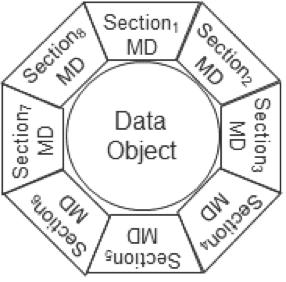
\includegraphics[width=0.25\textwidth]{fig/object.png}
  \caption{Object with Metadata Partitions}
  \label{fig:object}
\end{figure}

Finally, it's critical that an \os{} can scale---not just in its ability to store petabytes of data, but to be able to keep track of billions of discrete objects and associated \md{}. The former is comparatively easy, the latter is far more difficult. With HCP, each node can independently manage in excess of 800 million data objects and associated \md{}, a full cluster can manage 64 billion.
